\documentclass[ignorenonframetext,]{beamer}
\setbeamertemplate{caption}[numbered]
\setbeamertemplate{caption label separator}{: }
\setbeamercolor{caption name}{fg=normal text.fg}
\beamertemplatenavigationsymbolsempty
\usepackage{lmodern}
\usepackage{amssymb,amsmath}
\usepackage{ifxetex,ifluatex}
\usepackage{fixltx2e} % provides \textsubscript
\ifnum 0\ifxetex 1\fi\ifluatex 1\fi=0 % if pdftex
\usepackage[T1]{fontenc}
\usepackage[utf8]{inputenc}
\else % if luatex or xelatex
\ifxetex
\usepackage{mathspec}
\else
\usepackage{fontspec}
\fi
\defaultfontfeatures{Ligatures=TeX,Scale=MatchLowercase}
\fi
\usetheme{AnnArbor}
\usecolortheme{dolphin}
\usefonttheme{professionalfonts}
% use upquote if available, for straight quotes in verbatim environments
\IfFileExists{upquote.sty}{\usepackage{upquote}}{}
% use microtype if available
\IfFileExists{microtype.sty}{%
\usepackage{microtype}
\UseMicrotypeSet[protrusion]{basicmath} % disable protrusion for tt fonts
}{}
\newif\ifbibliography
\usepackage{longtable,booktabs}
\usepackage{caption}
% These lines are needed to make table captions work with longtable:
\makeatletter
\def\fnum@table{\tablename~\thetable}
\makeatother

% Prevent slide breaks in the middle of a paragraph:
\widowpenalties 1 10000
\raggedbottom

\AtBeginPart{
\let\insertpartnumber\relax
\let\partname\relax
\frame{\partpage}
}
\AtBeginSection{
\ifbibliography
\else
\let\insertsectionnumber\relax
\let\sectionname\relax
\frame{\sectionpage}
\fi
}
\AtBeginSubsection{
\let\insertsubsectionnumber\relax
\let\subsectionname\relax
\frame{\subsectionpage}
}

\setlength{\parindent}{0pt}
\setlength{\parskip}{6pt plus 2pt minus 1pt}
\setlength{\emergencystretch}{3em}  % prevent overfull lines
\providecommand{\tightlist}{%
\setlength{\itemsep}{0pt}\setlength{\parskip}{0pt}}
\setcounter{secnumdepth}{0}


% \pgfdeclareimage[width=1cm]{logo}{./figures/monkeyTypewriter.png}
%\logo{\pgfuseimage{logo}}

\institute{University of Virginia}
\definecolor{links}{RGB}{42, 27, 129}
\definecolor{mypink2}{RGB}{219, 48, 122}
%\hypersetup{colorlinks,linkcolor=links,urlcolor=mypink2}
\usefonttheme{professionalfonts}

% \setbeamerfont{note page}{family*=pplx,size=\footnotesize} % Palatino for notes

\setbeamerfont{subtitle}{size=\small}

\definecolor{uvablue}{RGB}{0,85,150}
\definecolor{uvalibraryorange}{RGB}{252,175,23}
\definecolor{uvacream}{RGB}{241,229,199}
\definecolor{uvalightblue}{RGB}{163,220,230}

\setbeamercolor{block body}{bg=green,fg=green}
\setbeamercolor{block body alerted}{bg=green,fg=green}
\setbeamercolor{block body example}{bg=green,fg=green}

\setbeamercolor{caption name}{fg=uvablue}

\setbeamercolor{headline}{fg=uvacream,bg=uvacream}
\setbeamercolor{section}{fg=uvalibraryorange,bg=uvablue}
\setbeamercolor{frametitle}{fg=uvalibraryorange,bg=uvablue}
\setbeamercolor{palette primary}{bg=uvalibraryorange,fg=uvablue}
\setbeamercolor{palette secondary}{bg=uvablue,fg=uvablue}
\setbeamercolor{palette tertiary}{bg=uvalibraryorange,fg=uvablue}
\setbeamercolor{palette quarternary}{fg=uvalibraryorange,bg=uvablue}
\setbeamercolor{palette sidebar primary}{bg=uvalibraryorange,fg=uvablue}
\setbeamercolor{palette sidebar secondary}{fg=uvablue,bg=uvablue}
\setbeamercolor{palette sidebar tertiary}{fg=uvalibraryorange,bg=uvablue}
\setbeamercolor{palette sidebar quarternary}{fg=uvalibraryorange,bg=uvablue}
\setbeamercolor{structure}{bg=uvablue}



\useinnertheme{rectangles}

\titlegraphic{\vspace{-7.5mm}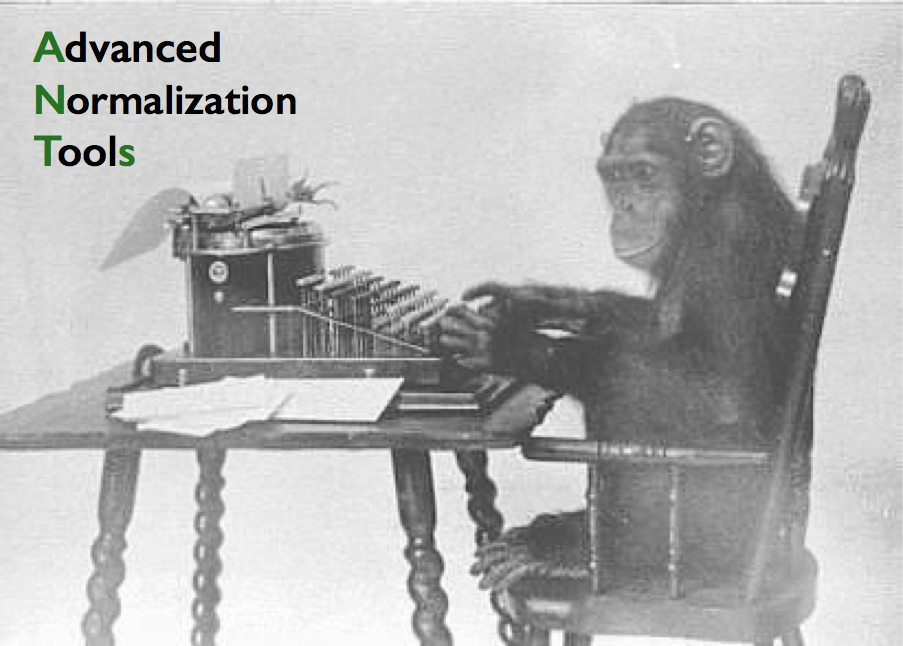
\includegraphics[width=0.45\paperwidth]{./figures/monkeyTypewriter.png}}

\title{Quantitative neuroimaging with ANTs}
\author{Nick Tustison}
\date{}

\begin{document}
\frame{\titlepage}

\begin{frame}

\end{frame}

\section{What is ANTs?}\label{what-is-ants}

\begin{frame}{NLM's The Visible Human Project and The Insight Toolkit}

\begin{center}

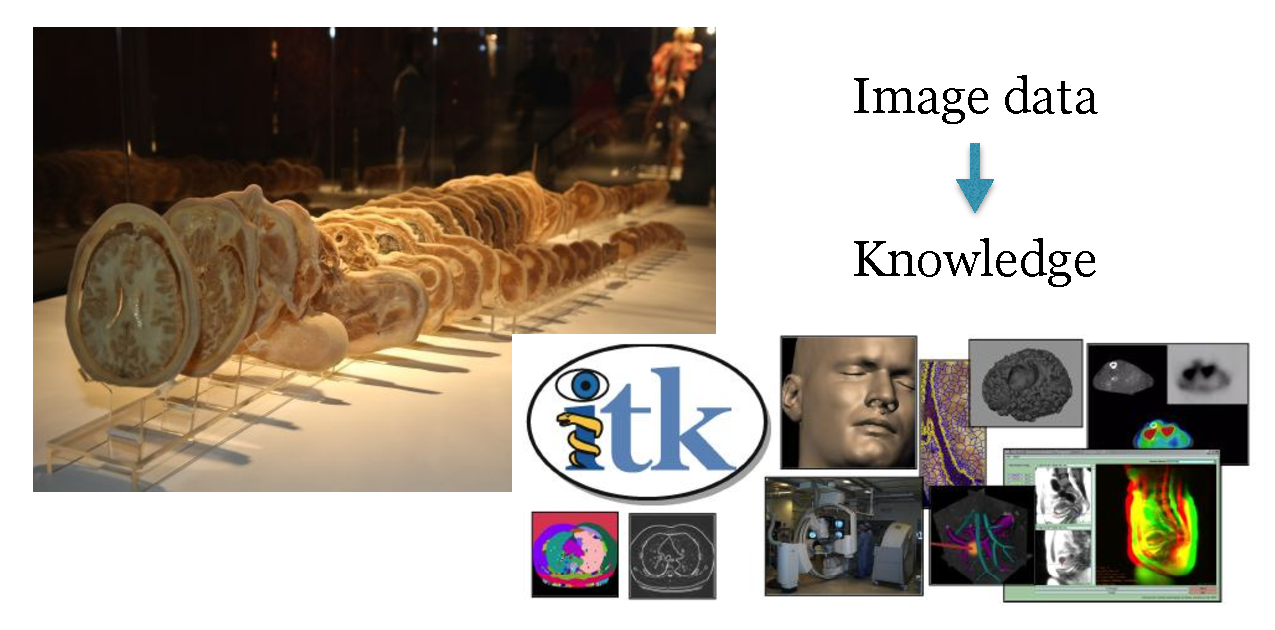
\includegraphics[width=4.75in]{./figures/VisibleHumanProject_ITK.pdf}

\end{center}

\end{frame}

\begin{frame}{ANTs \emph{began with a clinical research need.}}

\begin{center}

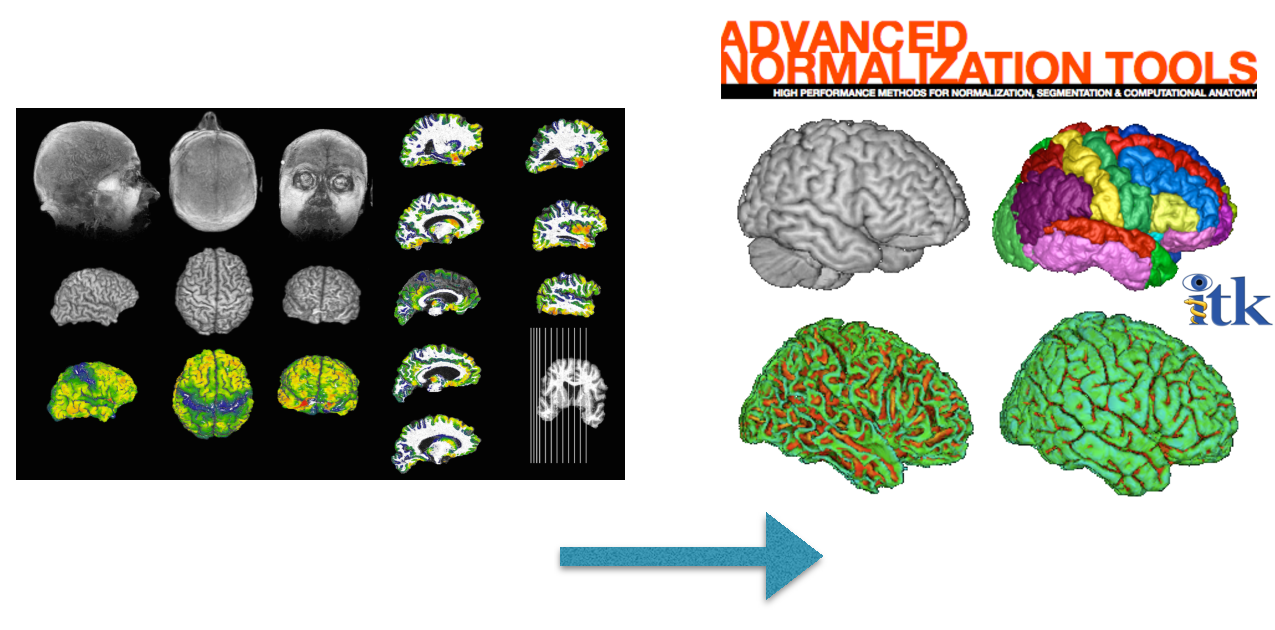
\includegraphics[width=4.75in]{./figures/ANTsEvolutionarySummary.pdf}

\end{center}

\end{frame}

\begin{frame}{Advanced Normalization Tools}

\begin{center}

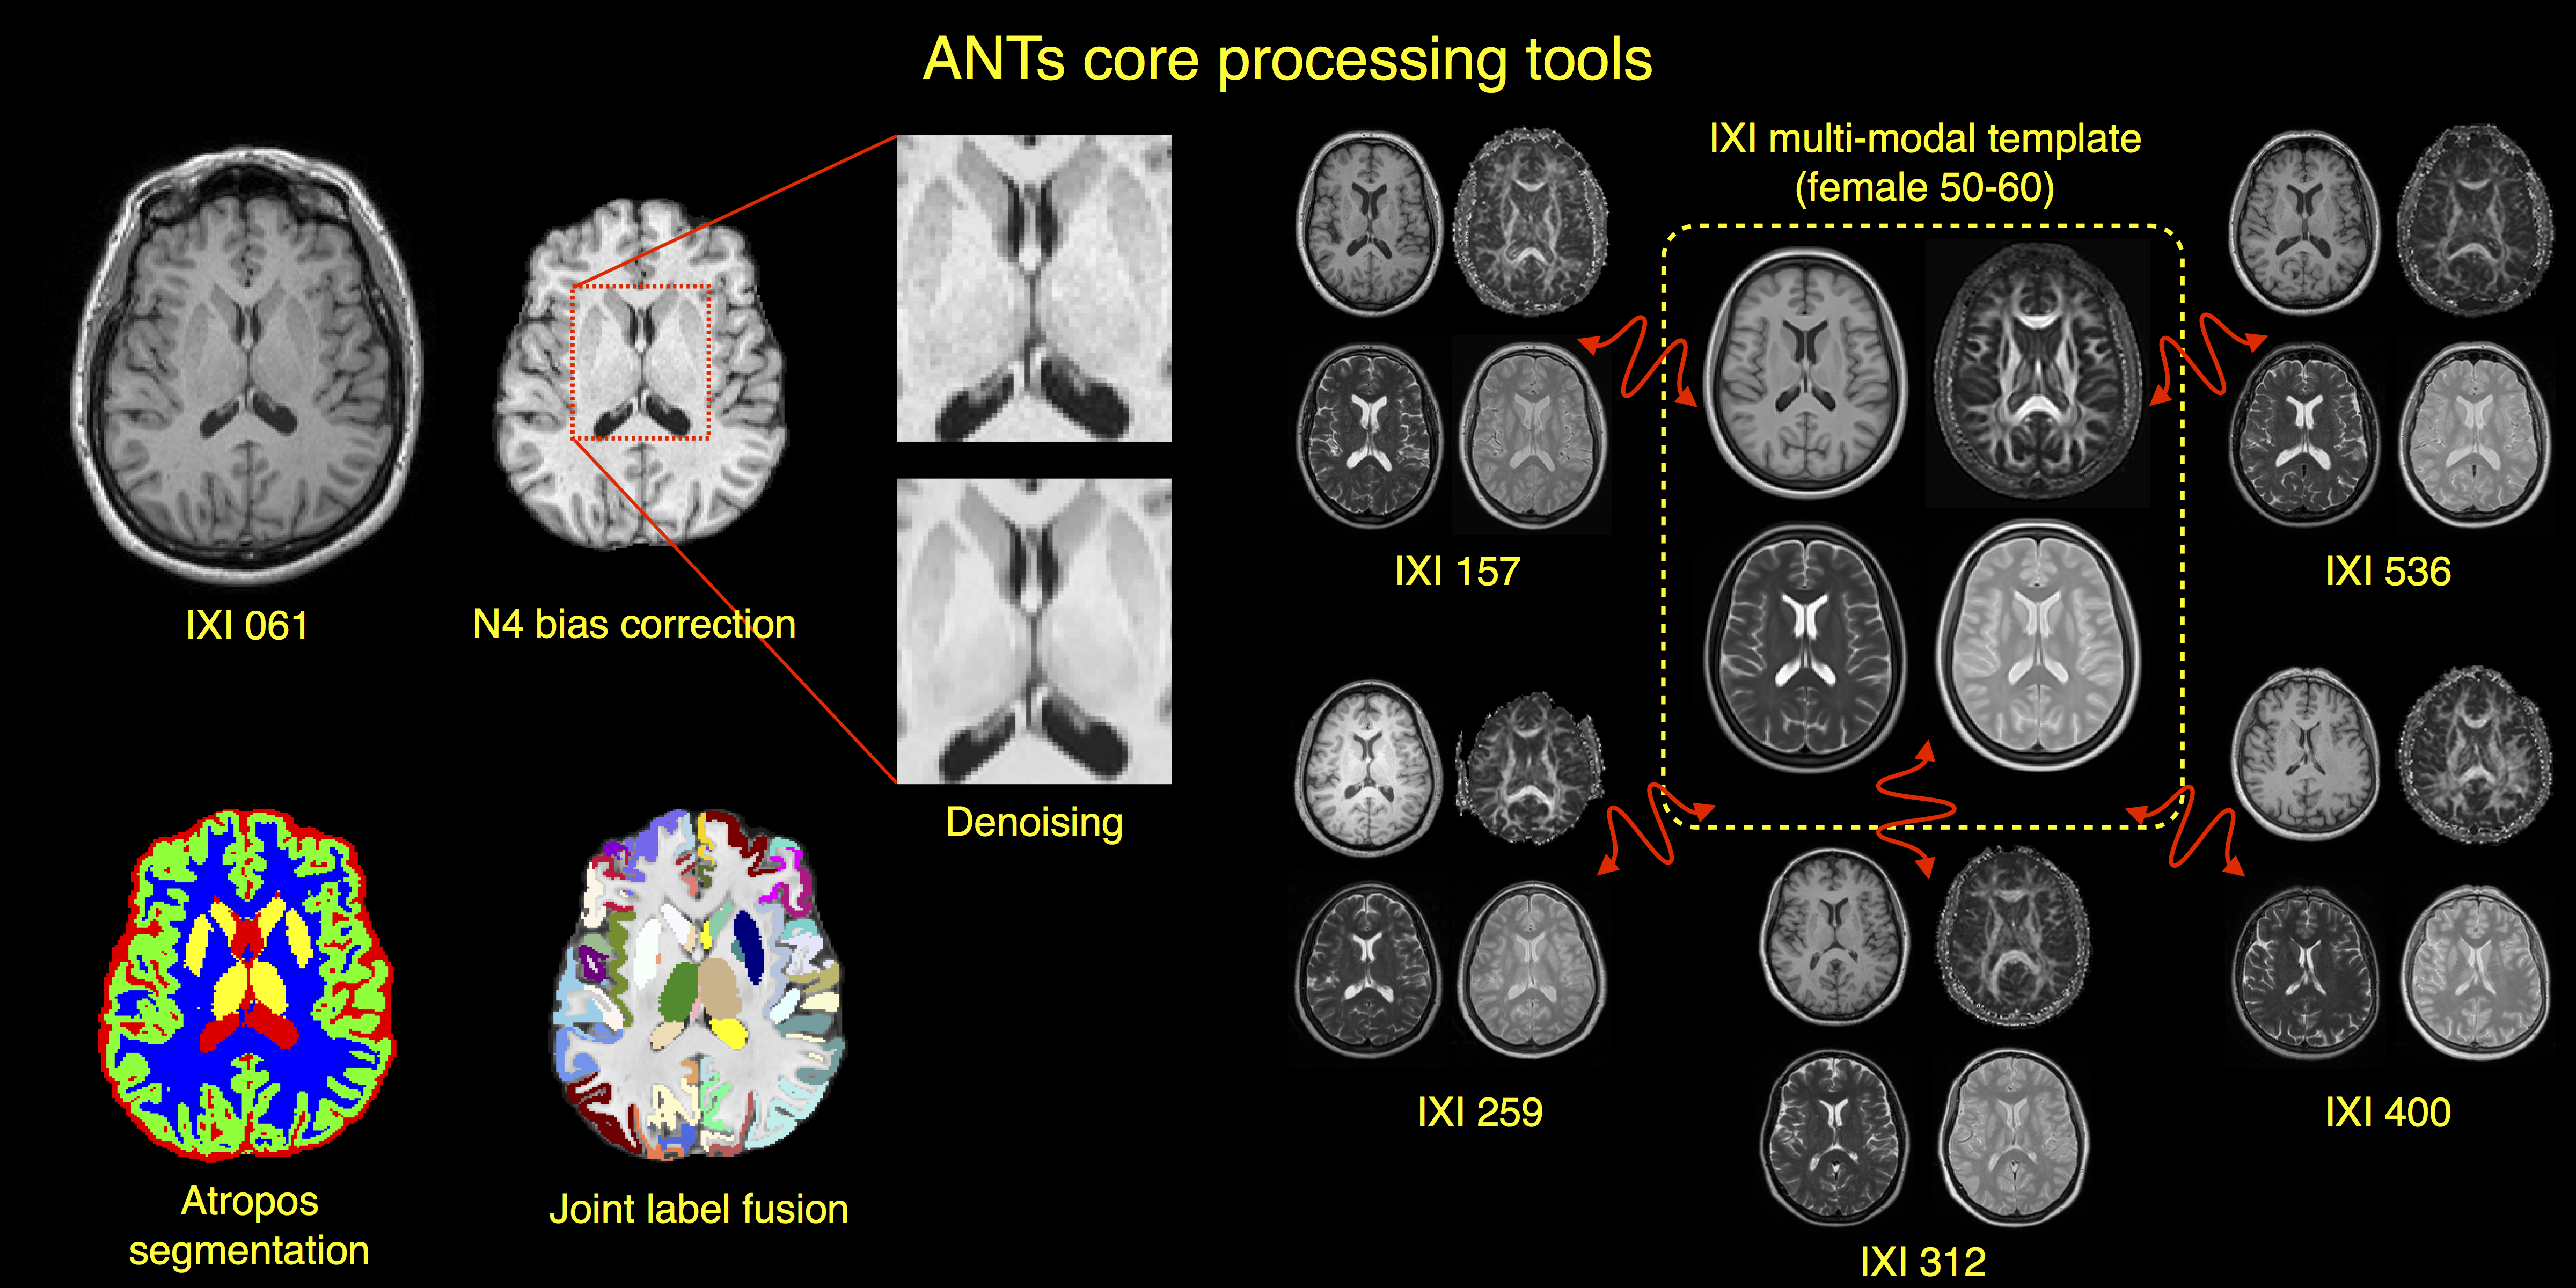
\includegraphics[width=4.75in]{./tools/figures/coreANtsToolsNeuro.png}

\end{center}

\end{frame}

\begin{frame}{Advanced Normalization Tools \(\rightarrow\) ``ITK-Lung''}

\begin{center}

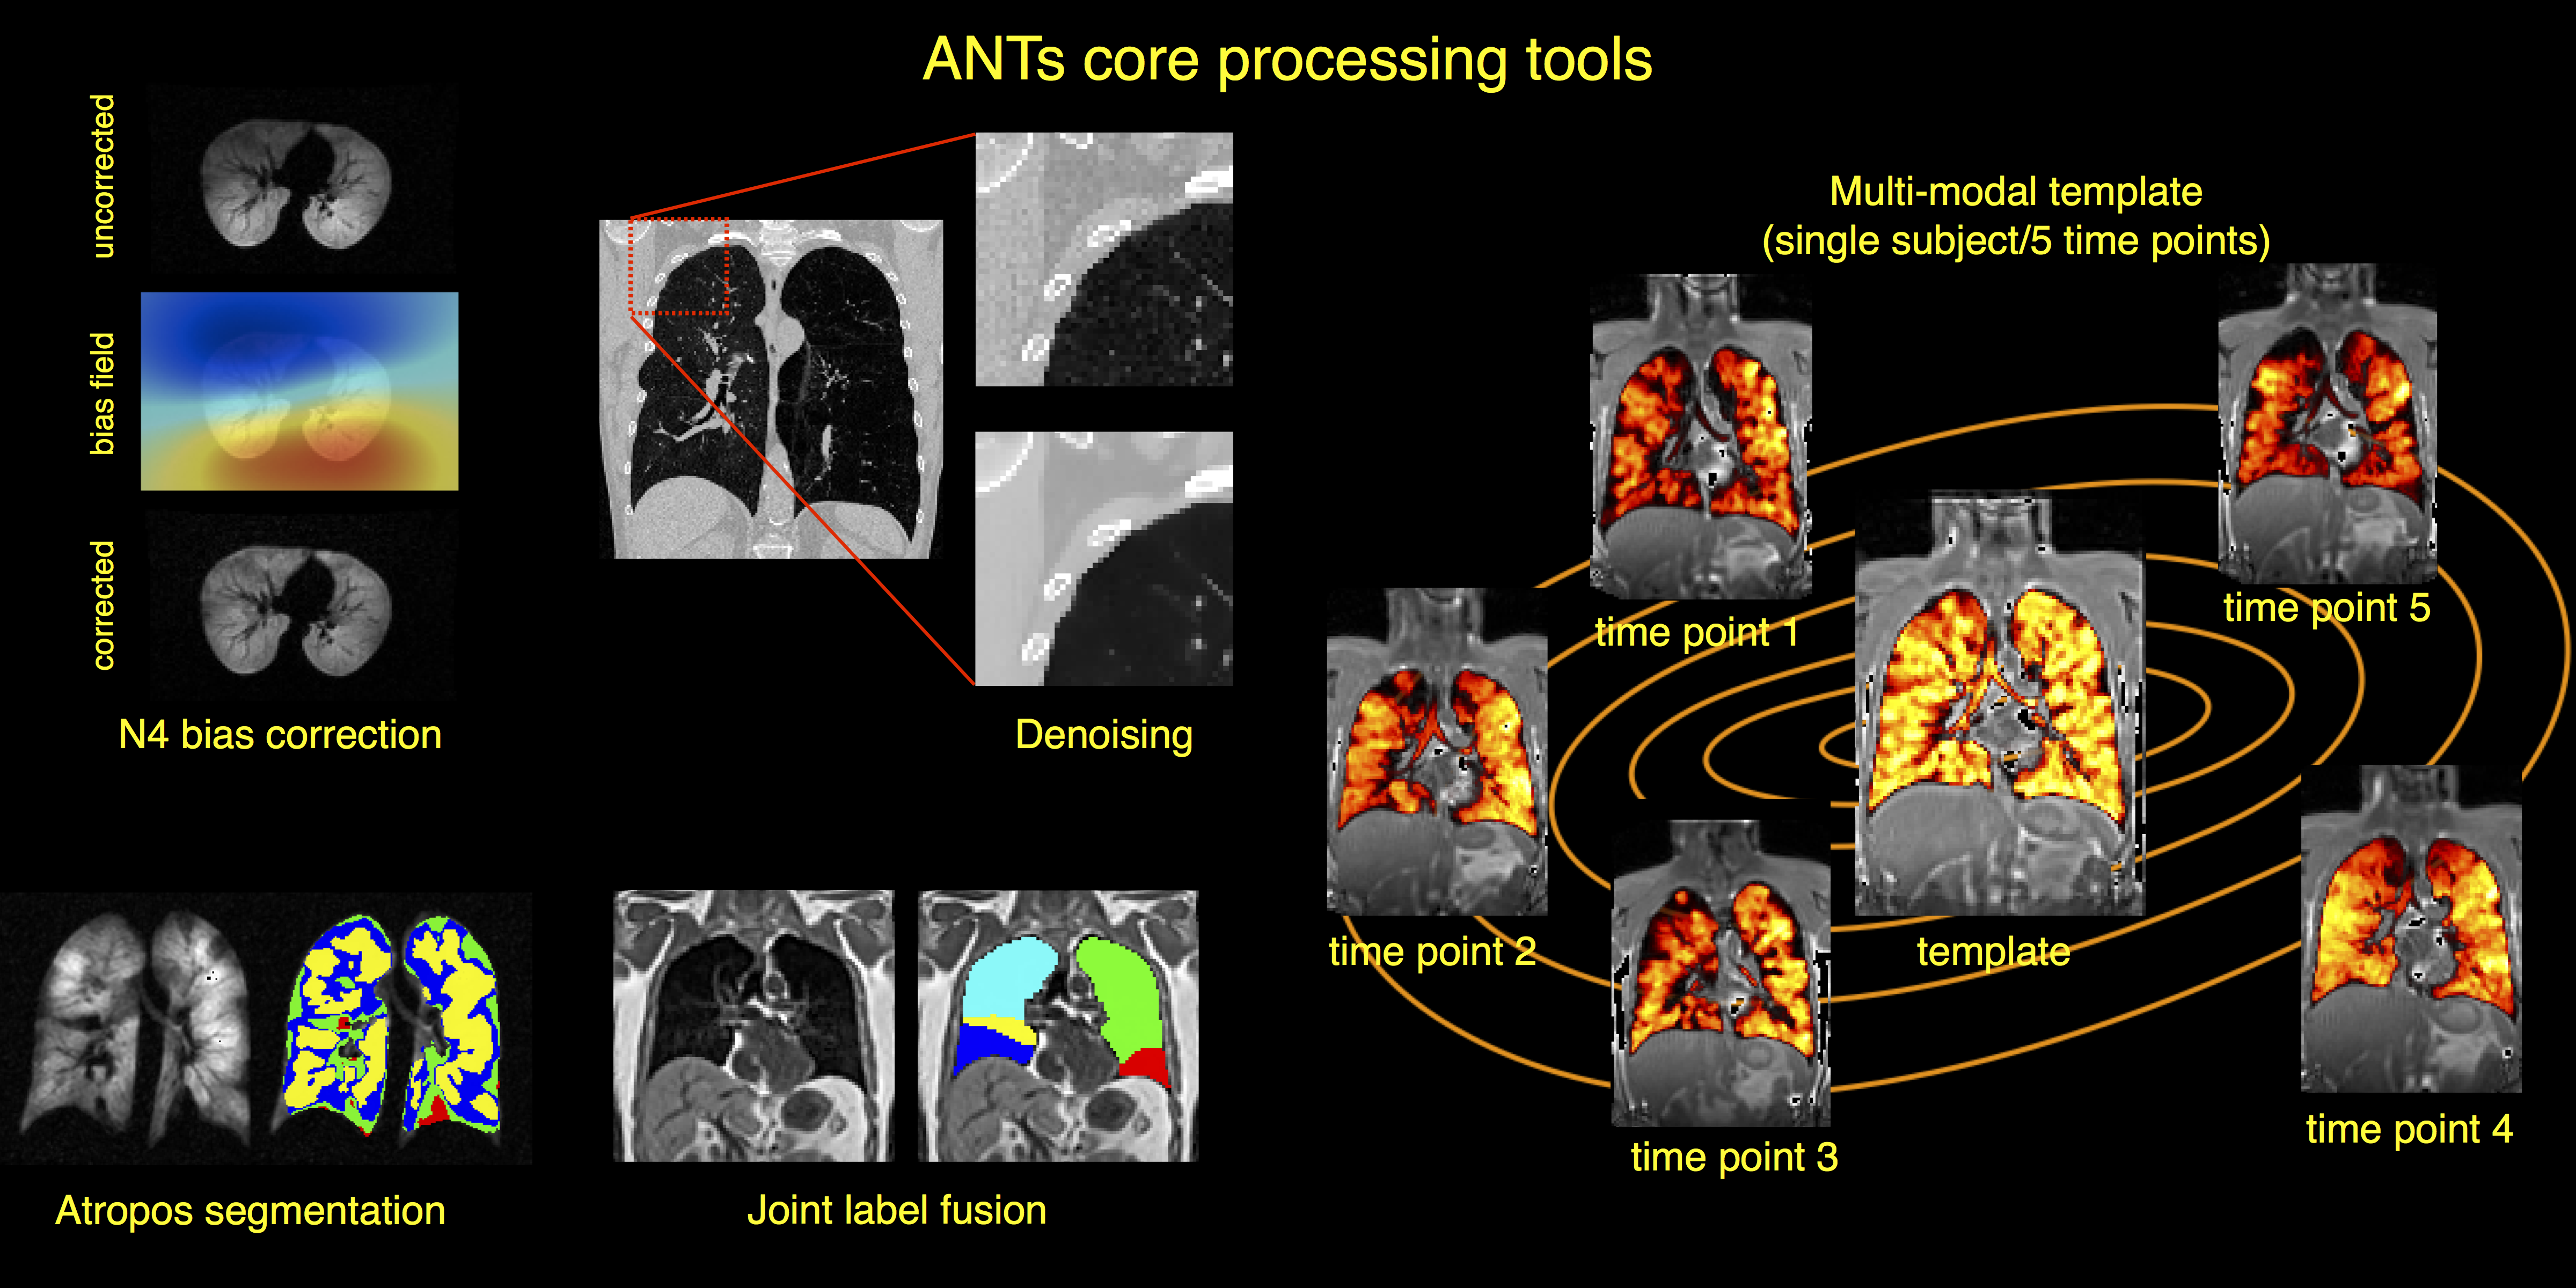
\includegraphics[width=4.75in]{./tools/figures/coreANtsToolsLung.png}

\end{center}

\end{frame}

\begin{frame}{International competitions}

\begin{itemize}
\item
  \href{http://www.ncbi.nlm.nih.gov/pubmed/19195496}{Klein 2009}: MRI
  brain registration
\item
  \href{http://empire10.isi.uu.nl}{EMPIRE 2010}: CT lung registration
\item
  \href{https://masi.vuse.vanderbilt.edu/workshop2012/index.php/Main_Page}{Multi-Atlas
  Label Challenge 2012}: MRI brain registration and segmentation
\item
  \href{https://masi.vuse.vanderbilt.edu/workshop2013/index.php/MICCAI_2013_SATA_Challenge_and_Workshop:Current_events}{SATA
  Challenge 2013}: MRI cardiac and canine hind leg registration
\item
  \href{http://martinos.org/qtim/miccai2013/}{BRATS 2013}: Multi-modal
  MRI brain segmentation
\item
  \href{http://www.cardiacatlas.org/web/stacom2014/moco-introduction}{STACOM
  2014 MoCo Challenge}: MRI cardiac motion estimation
\end{itemize}

\end{frame}

\section{Putting it all together---the ANTs cortical thickness
pipeline}\label{putting-it-all-togetherthe-ants-cortical-thickness-pipeline}

\begin{frame}{Cortical thickness studies}

\scriptsize

\begin{longtable}[c]{@{}ll@{}}
\toprule
Column1 & Column2\tabularnewline
\midrule
\endhead
Tetris-playing ability & chronic pancreatitis\tabularnewline
Huntington's disease & obsessive-compulsive disorder\tabularnewline
schizophrenia & ADHD\tabularnewline
bipolar disorder & obesity\tabularnewline
Alzheimer's disease & heritable depression\tabularnewline
frontotemporal dementia & elderly depression\tabularnewline
Parkinson's disease & age\tabularnewline
Williams syndrome & gender\tabularnewline
multiple sclerosis & handedness\tabularnewline
autism & intelligence\tabularnewline
migraines & athletic ability\tabularnewline
chronic smoking & meditative practices\tabularnewline
alcoholism & musical ability\tabularnewline
cocaine addiction & tendency toward criminality\tabularnewline
Tourette syndrome in children & childhood sexual abuse in female
adolescents\tabularnewline
scoliosis in female adolescents & traumatic brain injury\tabularnewline
early-onset blindness & untreated male-to-female
transsexuality\tabularnewline
\bottomrule
\end{longtable}

\end{frame}

\begin{frame}{The ANTs structural brain mapping workflow}

\begin{centering}

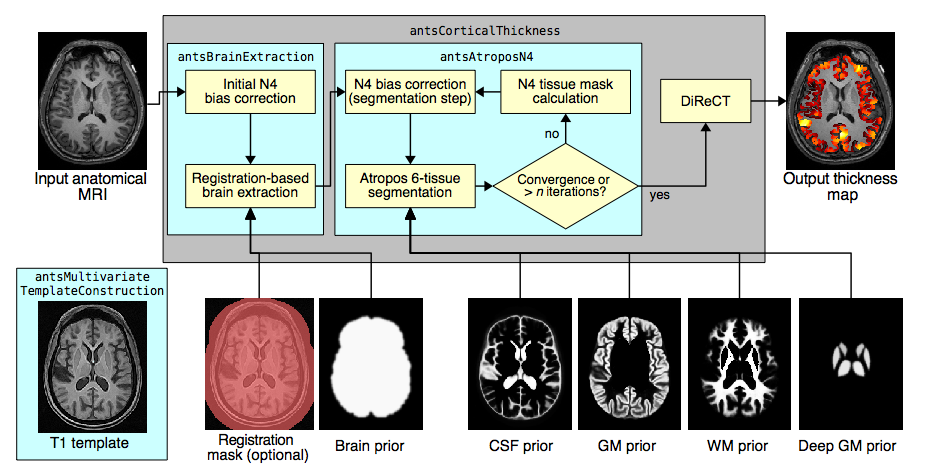
\includegraphics[width=4.5in]{./evaluation/figures/pipeline.png}

\end{centering}

\end{frame}

\begin{frame}{Template building}

\emph{Tailor data to your specific cohort}

\begin{centering}

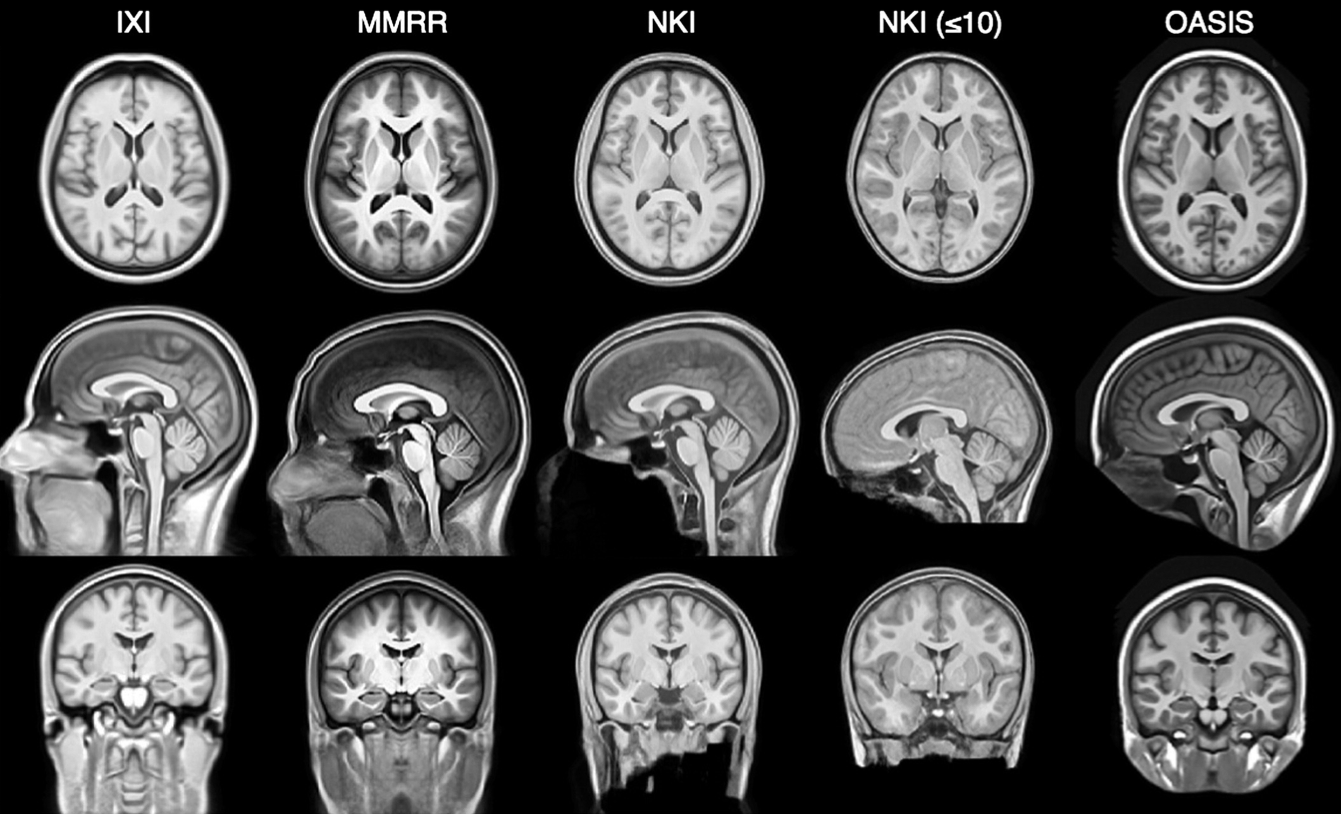
\includegraphics[width=3in]{./evaluation/figures/templates.png}

\end{centering}

\small

\begin{itemize}
\tightlist
\item
  Templates representing the average mean shape and intensity are built
  directly from the cohort to be analyzed, e.g.~pediatric
  vs.~middle-aged brains.\\
\item
  Acquisition and anonymization (e.g.~defacing) protocols are often
  different.
\end{itemize}

\end{frame}

\begin{frame}{Template priors}

\begin{centering}

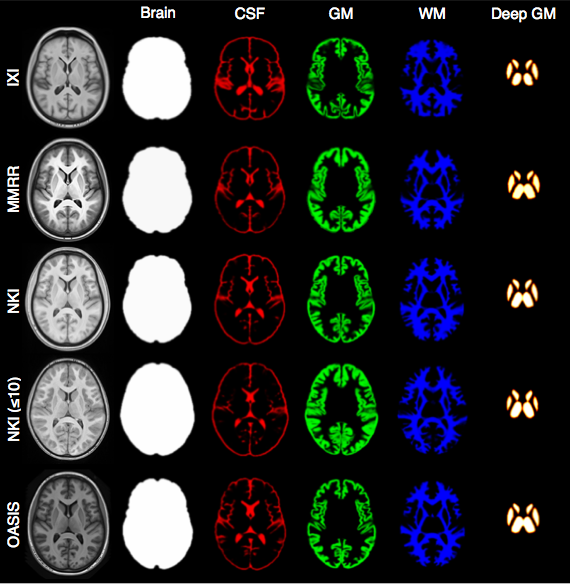
\includegraphics[width=2.5in]{./evaluation/figures/templatePriors.png}

\end{centering}

\small

Each template is
\href{https://github.com/ntustison/antsCookTemplatePriorsExample}{processed}
to produce auxiliary images which are used for brain extraction and
brain segmentation.

\end{frame}

\begin{frame}{Brain extraction comparison}

\begin{centering}

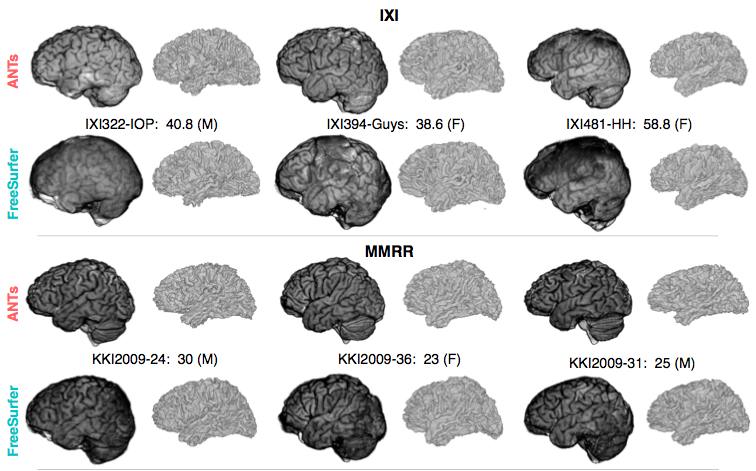
\includegraphics[width=3.5in]{./evaluation/figures/brainExtraction.png}

\end{centering}

\small

Comparison with de facto standard FreeSurfer package. Note the
difference in separation of the gray matter from the surrounding CSF. (0
failures out of 1205 scans)

\end{frame}

\begin{frame}[fragile]{Brain segmentation}

\begin{centering}

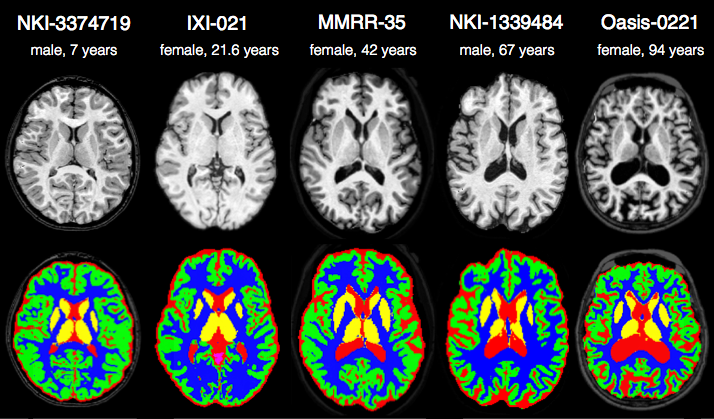
\includegraphics[width=3.5in]{./evaluation/figures/brainSegmentation.png}

\end{centering}

\small

Randomly selected healthy individuals. \texttt{Atropos} gets good
performance across ages.

\end{frame}

\begin{frame}{Cortical thickness maps}

\begin{centering}

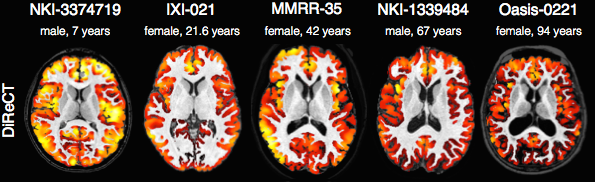
\includegraphics[width=4in]{./evaluation/figures/corticalThicknessEstimation.png}

\end{centering}

\small

In contrast to FreeSurfer which warps coupled surface meshes to segment
the gray matter, \emph{ANTs} diffeomorphically registers the white
matter to the combined gray/white matters while simultaneously
estimating thickness.

\end{frame}

\begin{frame}

\begin{centering}

\Large

{\bf But without ground truth, how does one evaluate the pipeline?}

\end{centering}

\end{frame}

\begin{frame}{Predict age and gender}

\begin{centering}

$AGE \sim VOLUME + GENDER + \sum_{i=1}^{62} T(DKT_i)$

\end{centering}

\end{frame}

\begin{frame}{Prediction from cortical thickness data}

\begin{centering}

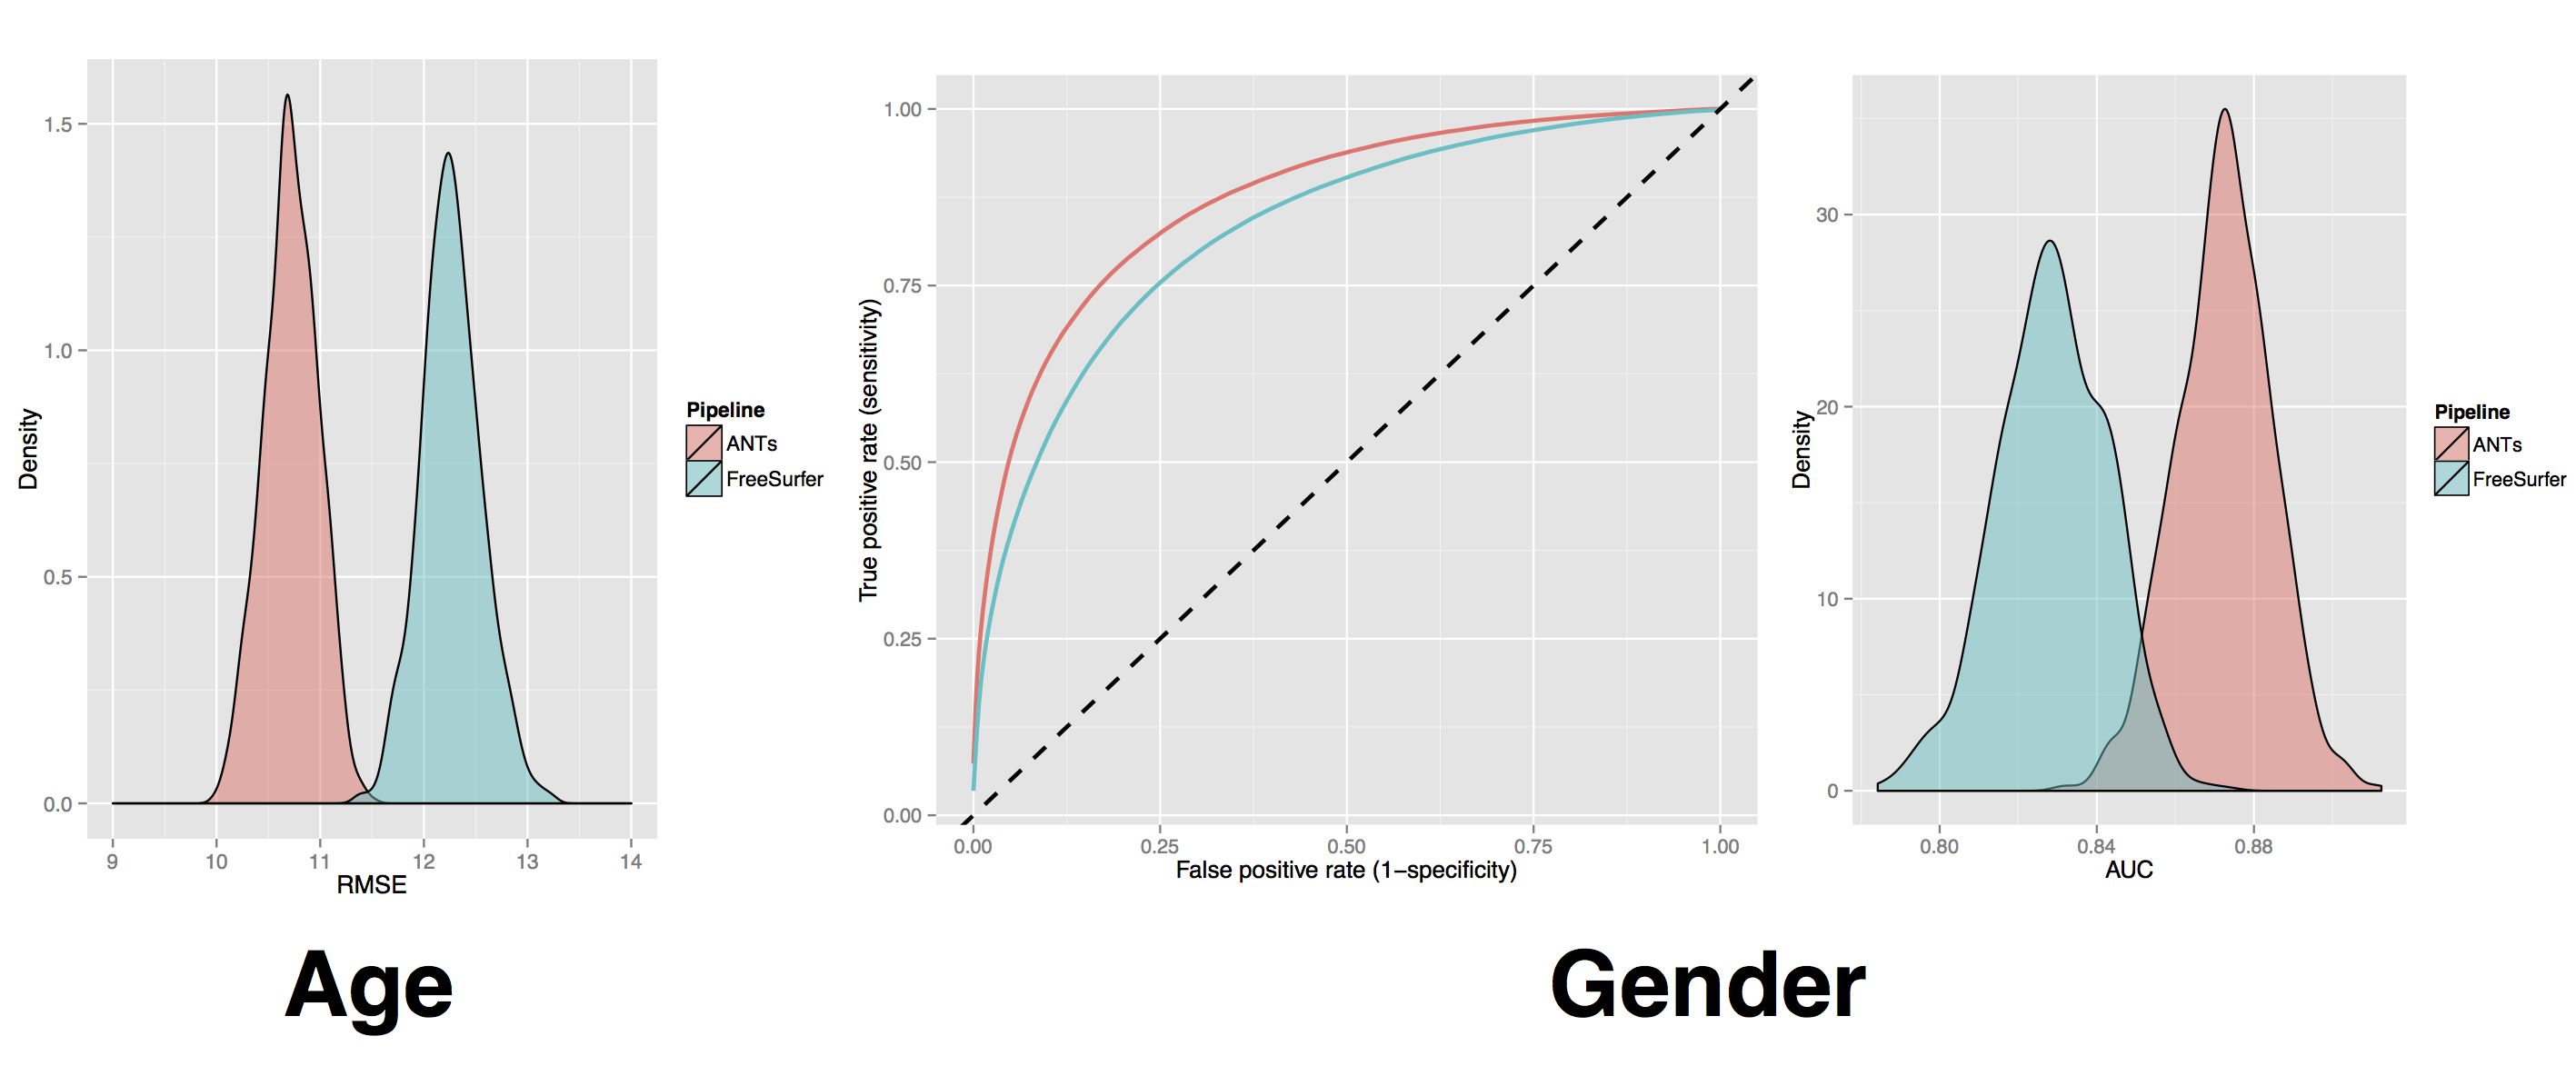
\includegraphics[width=4in]{./evaluation/figures/evaluation.png}

\end{centering}

\end{frame}

\begin{frame}{Regional importance comparison}

\begin{centering}

\small
ANTs (left) vs. FreeSurfer (right)

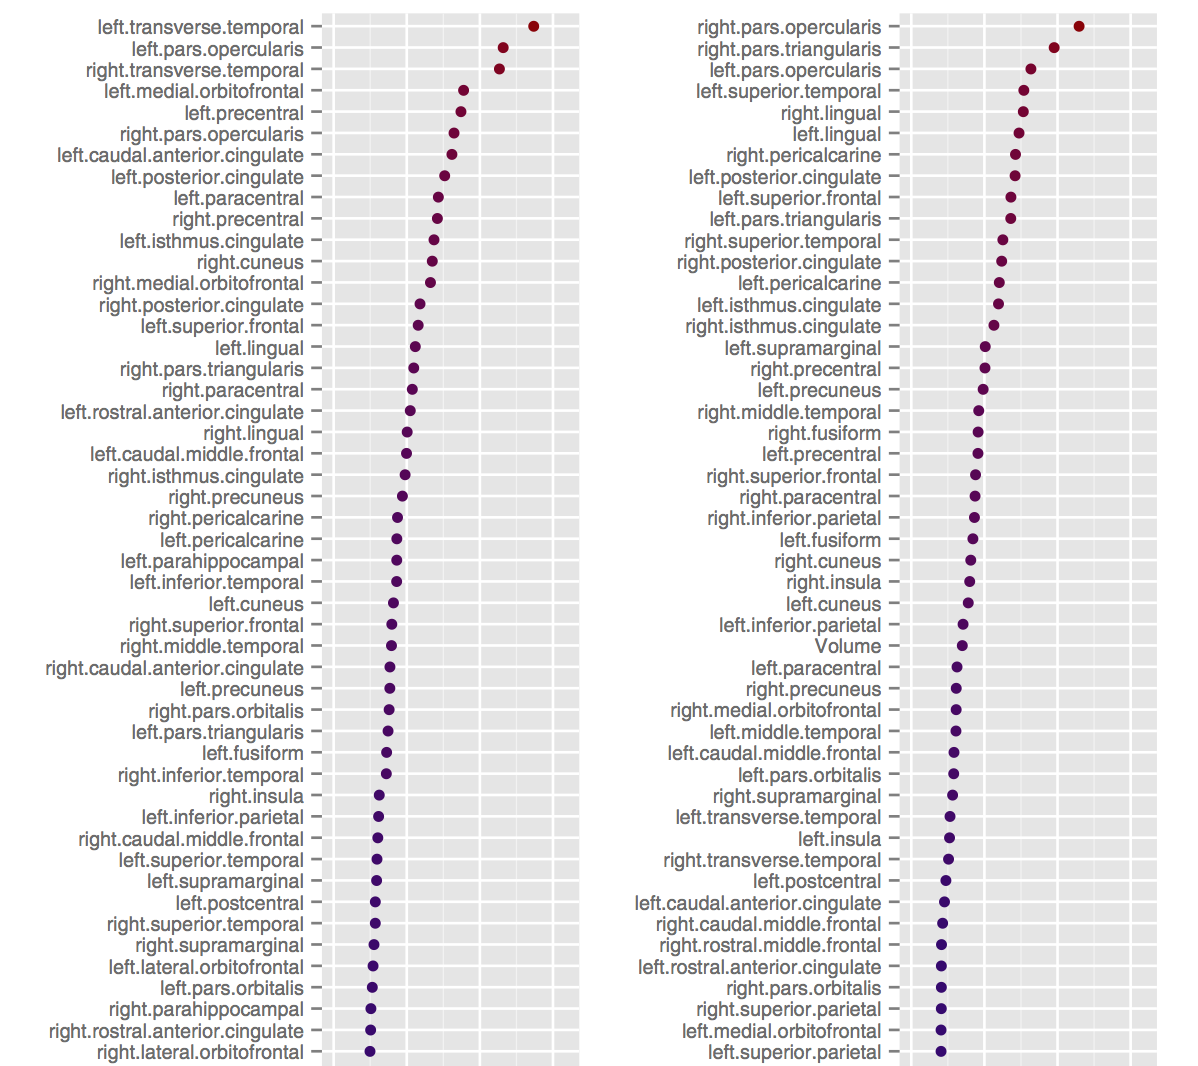
\includegraphics[width=4in]{./evaluation/figures/antsvfreesurfer_Importance.png}

\end{centering}

\end{frame}

\section{Advanced Normalization Tools in R
(ANTsR)}\label{advanced-normalization-tools-in-r-antsr}

\begin{frame}{Multimodal Brain Tumor Segmentation (BRATS 2013)}

\begin{centering}

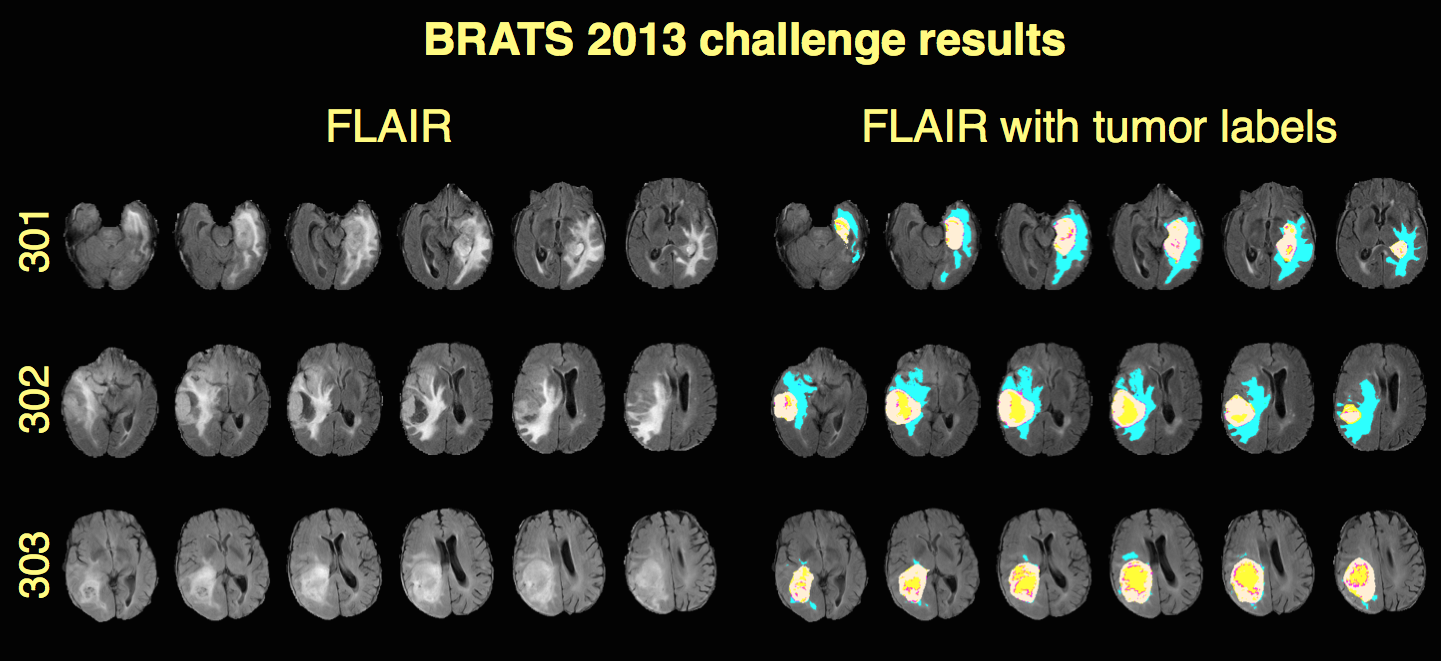
\includegraphics[width=4.5in]{./competitions/figures/brats2013results1.png}

\end{centering}

\small

\href{http://www.ncbi.nlm.nih.gov/pubmed/25433513}{Tustison, et al.,
Optimal symmetric multimodal templates and concatenated random forests
for supervised brain tumor segmentation (simplified) with \emph{ANTsR},
\emph{Neuroinformatics}.}

\end{frame}

\begin{frame}{White matter hyperintensities in TBI}

\begin{centering}

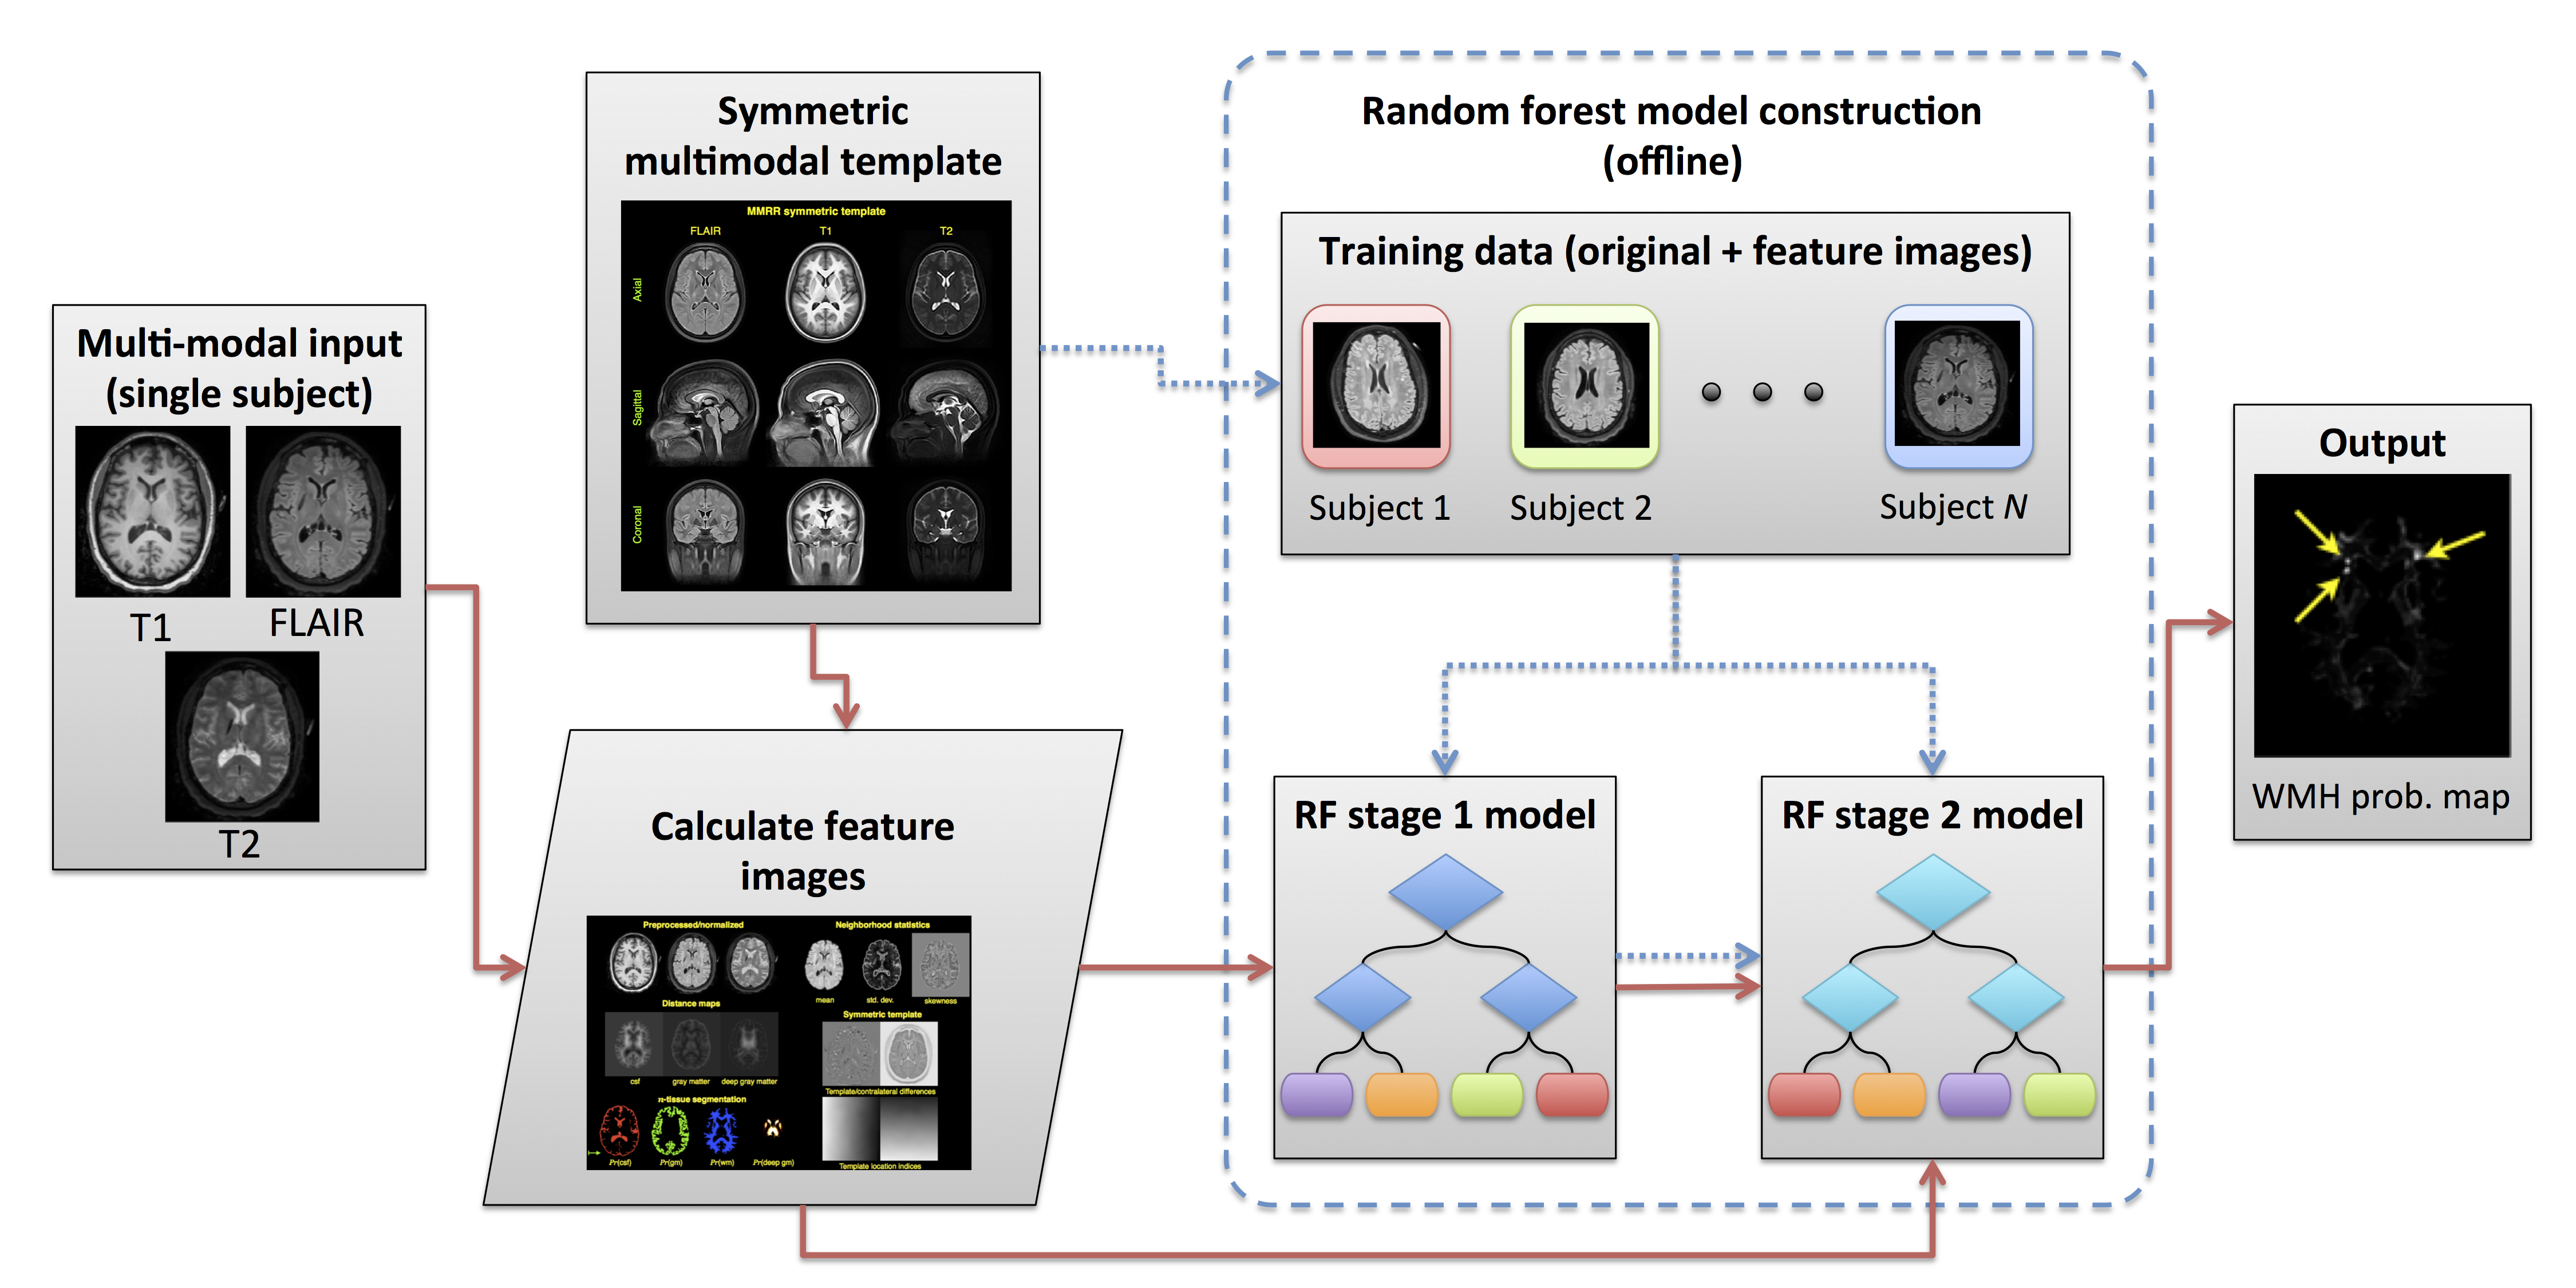
\includegraphics[width=4.5in]{./wmhs/figures/wmhPipeline.png}

\end{centering}

\end{frame}

\begin{frame}{Social behavior and immunity dysfunction in mice}

\begin{centering}

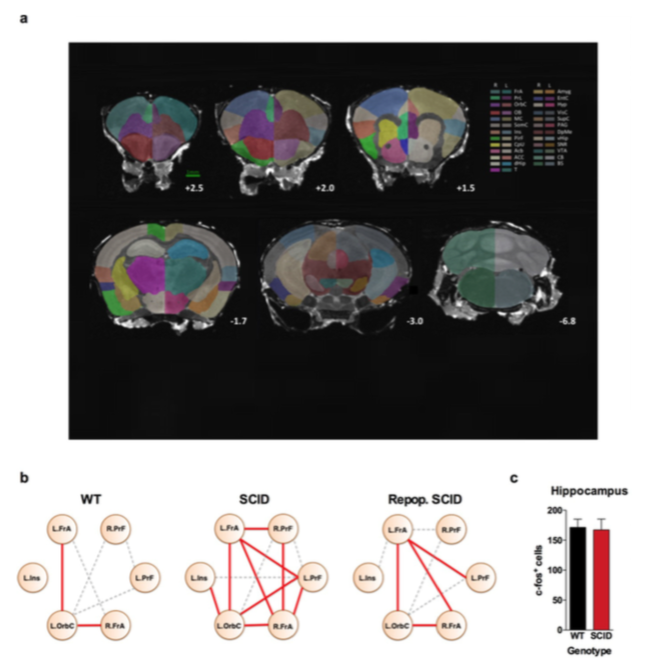
\includegraphics[width=3in]{./antsr/figures/filiano_rsfmri.png}

\end{centering}

\end{frame}

\begin{frame}{Other ANTsR work}

\begin{itemize}
\item
  \href{http://www.nature.com/articles/sdata20153}{Pediatric template of
  brain perfusion}
\item
  \href{http://www.ncbi.nlm.nih.gov/pubmed/26756101}{Automated
  segmentation of chronic stroke lesions using LINDA: Lesion
  identification with neighborhood data analysis}
\item
  \href{http://www.ncbi.nlm.nih.gov/pubmed/25448483}{Eigenanatomy}
\item
  Corrective learning for segmentation refinement
\end{itemize}

\end{frame}

\begin{frame}{Open source}

\begin{itemize}
\tightlist
\item
  \url{https://github.com/stnava/ANTs}
\item
  \url{https://github.com/stnava/ANTsR}
\end{itemize}

\hypertarget{refs}{}

\end{frame}

\end{document}
